\setcounter{section}{2}
\section{Rigid Body Dynamics}
\setcounter{section}{6}
\setcounter{subsection}{11}
\subsection{Kinematics of a rigid body} %% ----------------- 6 . 12 ------------
\(\vec{\omega}_{io}\) is the angular velocity of the \(o\) frame with respect to the \(i\) frame.

\({}^i\frac{d}{dt}\vec{r}_o\) is the derivative of \(\vec{r}_o\) in the \(i\) frame.

\begin{Figure}
    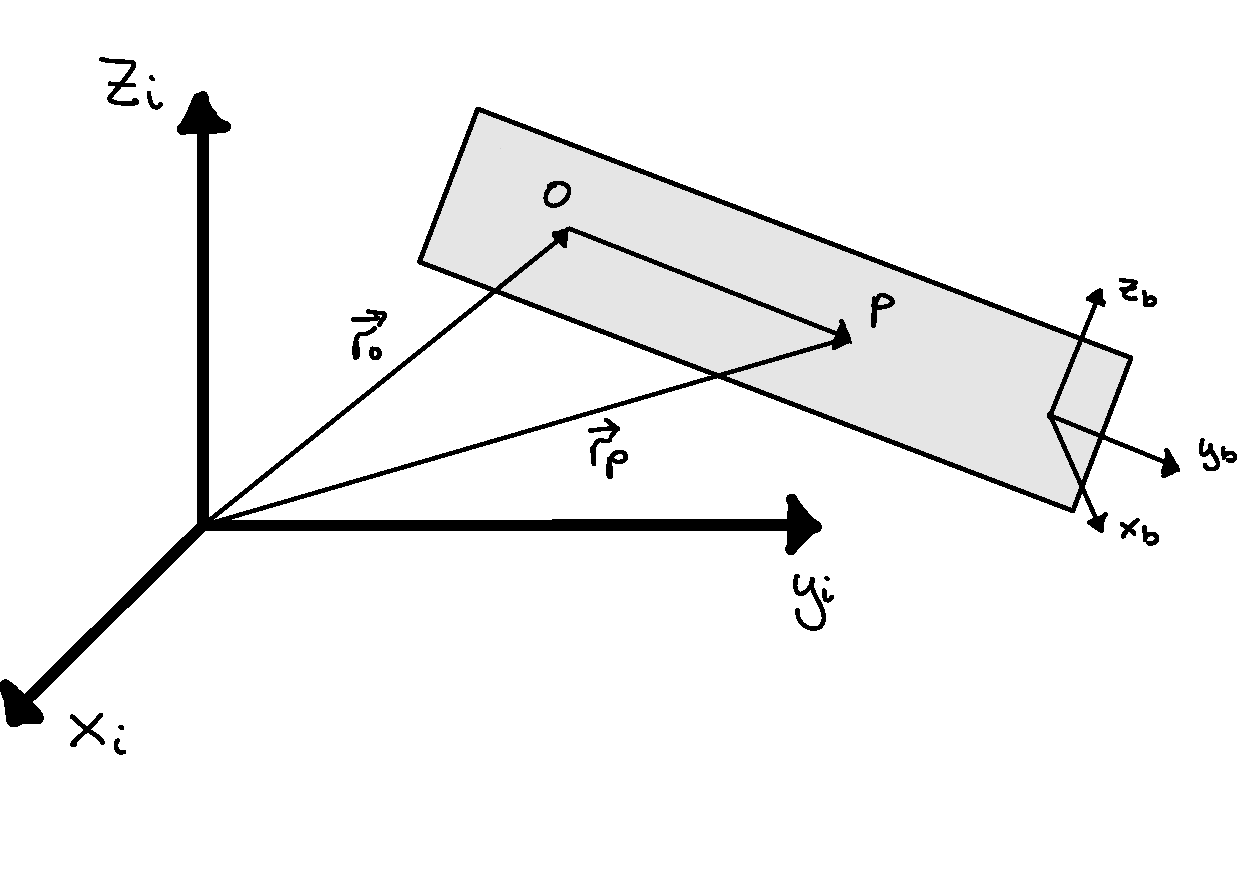
\includegraphics[clip, trim = 0cm 2cm 0cm 0cm,width=\linewidth]{figures/rigid-body.pdf}
    \label{fig:rigid-body}
\end{Figure}

Velocity and Acceleration
\begin{align*}
    \vec{v}_p &:= \frac{{}^id}{dt}\vec{r}_p \\
              &= \vec{v}_o + \frac{{}^bd}{dt}\vec{r} + \vec{\omega}_{ib}\times\vec{r} \\
    \vec{a}_p &:= \frac{{}^id^2}{dt^2}\vec{r}_p \\
              &= \vec{a}_o + \frac{{}^bd^2}{dt^2}\vec{r} + 2\vec{\omega}_{ib}\times\frac{{}^bd}{dt}\vec{r} + \vec{\alpha}_{ib}\times\vec{r} + \vec{\omega}_{ib}\times(\vec{\omega}_{ib}\times\vec{r})
\end{align*}
The last three terms are, respectively, the coriolis acceleration, Transversal acceleration and Centripetal acceleration. Note that
\begin{align*}
    \vec{a}_o = \frac{{}^id}{dt}\vec{v}_o = \frac{{}^bd}{dt}\vec{v}_o + \vec{\omega}_{ib}\times\vec{v}_o
\end{align*}



\subsection{The center of mass} %% ------------------------- 6 . 13 ------------

The center of mass of a rigid body \(\mathcal{C}\) is defined to be
\begin{align*}
    \vec{r}_c := \frac{1}{m}\int_{\mathcal{C}}\vec{r}_p\,dm
\end{align*}
It can be shown that
\begin{align*}
    \vec{v}_c &= \frac{1}{m}\int_{\mathcal{C}}\vec{v_p}\,dm  &
    \vec{a}_c &= \frac{1}{m}\int_{\mathcal{C}}\vec{a_p}\,dm
\end{align*}
where \(c\) denotes \textit{center}



\setcounter{section}{7}
\setcounter{subsection}{1}
\subsection{Forces and torques} %% ------------------------- 7 . 2 -------------

\textbf{Moment}. The moment about a point \(P\) of the set \(S = \{F_j\}_{j\in[1,n_F]}\) for forces is
\begin{align*}
    \vec{N}_{S/P} = \sum_{j=1}^{n_F}\vec{r_{Pj}}\times \vec{F}_j
\end{align*}
Where \(\vec{r}_{Pj}\) is an arbitrary point along the line of action of \(\vec{F}_j\)
\newline


\textbf{Torque} is defined as the moment of the couple \(\mathcal{C}\). A couple being a set of forces with \(\bm{0}\) resultant force.
\newline

\subsection{Newton-Euler Equations for rigid bodies} %% ---- 7 . 3 -------------

\textbf{Angular Momentum}. The angular momentum of the body \(b\) about the point \(c\) is
\begin{align*}
    \bm{h}_{b/c} &= \int_\mathcal{B} \bm{r}\times\bm{v} \,dm \\
    &= \bm{M}_{b/c}\bm{\omega}_{ib} \\
    \bm{T}_{bc} &= \frac{d}{dt}\bm{h}_{b/c}
\end{align*}


\textbf{Rotational Inertia / The inertia dyadic}. The inertia matrix of the body \(b\) about the point \(c\) is
\begin{align*}
    \bm{M}_{b/c} &= - \int_b \bm{r}^\times\bm{r}^\times\,dm \\
    &= \int_b (\bm{r}^T\bm{r}\mathbb{I} - \bm{r}\bm{r}^T)\,dm\\
    &= \begin{pmatrix}
        \bm{I}_{xx} & -\bm{I}_{xy} & -\bm{I}_{xz} \\
        -\bm{I}_{xy} & \bm{I}_{yy} & -\bm{I}_{yz} \\
        -\bm{I}_{xz} & -\bm{I}_{yz} & \bm{I}_{zz} \\
    \end{pmatrix}
\end{align*}
Where \(\bm{r}\) is the distance vector from the point \(c\) to the mass element being integrated
\begin{align*}
    \bm{I}_{xx} &= \int_b y^2 + z^2  \,dm & \bm{I}_{xy} = \int_b xy \,dm \\
    \bm{I}_{yy} &= \int_b x^2 + z^2  \,dm & \bm{I}_{xz} = \int_b xz \,dm\\
    \bm{I}_{zz} &= \int_b x^2 + y^2  \,dm & \bm{I}_{yz} = \int_b yz \,dm
\end{align*}
\begin{align*}
    \bm{M}_{b/c}^i = \bm{R}_b^i\bm{M}_{b/c}^b\bm{R}_i^b
\end{align*}

\textbf{Equations of motion}. Let \(b\) denote body, \(i\) an inertial frame, \(c\) the center of mass of \(b\), \(\bm{F}_{bc}\) a resultant force acting on \(b\) with line of action through \(c\) and \(\bm{T}_{bc}\) the torque about \(c\). Then
\begin{align*}
    \bm{F}_{bc} &= m\bm{a}_c \\
    \bm{T}_{bc} &= \bm{M}_{b/c}\bm{\alpha}_{ib} + \bm{\omega}_{ib}\times(\bm{M}_{b/c}\bm{\omega}_{ib})
\end{align*}
On compact matrix form
\begin{align*}
    \begin{pmatrix} m\mathbb{I} & \bm{0} \\ \bm{0} & \bm{M}_{b/c}^b \end{pmatrix}
        \begin{pmatrix}\bm{a}_c^b \\ \bm{\alpha}_{ib}^b \end{pmatrix} + 
        \begin{pmatrix} \bm{0} \\ (\bm{\omega}_{ib}^b)^\times\bm{M}_{b/c}^b\bm{\omega}_{ib}^b\end{pmatrix} =
            \begin{pmatrix}\bm{F}_{bc}^b \\ \bm{T}_{b/c}^b\end{pmatrix} \\
    \begin{pmatrix} m\mathbb{I} & \bm{0} \\ \bm{0} & \bm{M}_{b/c}^b \end{pmatrix}
        \begin{pmatrix}\dot{\bm{v}}_c^b \\ \bm{\alpha}_{ib}^b \end{pmatrix} + 
            \begin{pmatrix} m(\bm{\omega}_{ib}^b)^\times\bm{v}_c^b \\ (\bm{\omega}_{ib}^b)^\times\bm{M}_{b/c}^b\bm{\omega}_{ib}^b\end{pmatrix} =
            \begin{pmatrix}\bm{F}_{bc}^b \\ \bm{T}_{b/c}^b\end{pmatrix}
\end{align*}

\textbf{Kinetic energy}. The kinetic energy of the body \(b\) in an inertial reference frame \(i\) is
\begin{align*}
    K = \frac{1}{2}m(\bm{v}_c^b)^T\bm{v}_c^b + \frac{1}{2}(\bm{\omega}_{ib}^b)^T\bm{M}_{b/c}^b\bm{\omega}_{ib}^b
\end{align*}

\textbf{The parallel axes theorem}. The inertia matrix of \(b\) about \(o\) is related to the inertia matrix of \(b\) about \(c\) according to
\begin{align*}
    \bm{M}_{b/o}^b &= \bm{M}_{b/c}^b-m(\bm{r}_g^b)^\times(\bm{r}_g^b)^\times \\
    &= \bm{M}_{b/c}^b+m(||\bm{r}_g^b||^2\mathbb{I}-\bm{r}_g^b(\bm{r}_g^b)^T)
\end{align*}
Where \(\bm{r}_g^b\) is the vector from \(c\) to \(o\)
